% PART III: RTX Project Q&A
\chapter{Frequently Asked Questions}
We list frequently asked questions with answers in this chapter.
\section{Processor Management}
This section contains the frequently asked questions and answers of the following topics:
\begin{itemize}
\item context switching,
\item scheduling and preemption .
\end{itemize}
\subsection{Context Switching}
\begin{itemize}
\item[{\bf Q1:}] {\bf In tutorial slides, it showed our processes as having 5 states: Ready, Blocked on Resource, Waiting for Message, Executing, and Interrupted. Will these five states be sufficient for our lab, or should we, for example, have a``New" state (as in the context switching sample code on GitHub)?} 
\item[A1:] The NEW state says a process which has never been run before is now ready to run. Tutorial slides are at a higher abstraction level. If you feel adding a new state will help you to manage the processor, then feel free to add more states. The NEW state on GitHub can be considered as a special READY state in tutorial slides.

\item[{\bf Q2:}] {\bf If a process completes itself without calling \verb+release_processor()+, should it be taken off the ready queue automatically? Should the next process be dispatched?}
\item[A2:] The project requires processes never terminate (i.e. they never exit). You can keeping calling the \verb+release_processor()+ after all useful actions are completed to prevent the process from terminating.  

\item[{\bf Q3:}] {\bf What does the \verb+__set_MSP()+ function do, and how is it able to update the program counter/link register to switch to a new process?}
\item[A3:] This function sets the MSP to the value supplied. Each process has its own stack, by switching between stacks, we achieve the purpose of context switching.

\item[{\bf Q4:}] {\bf How does saving/loading process contexts work in assembly code? Is there any part of the sample code which would help us understand this?}
\item[A4:] You will need to use assembly code to access C data structures. Section \ref{sec_asm_c} in the SE350 lab manual provides some code excerpts on this topic. The starter code \url{https://github.com/yqh/SE350/blob/master/manual_code/Context_Switching/src/k_process.c} shows how to context switch between two processes. Please be aware of the assumptions made at the beginning of the code comments block.

\item[{\bf Q5:}] {\bf Where to put the PCB priority queues?}
\item[A5:] The PCB queue structure memory can either be allocated at compile time (i.e. inside the image of your RTX) or at run time (i.e. when you do memory initialization in RTX.).

\item[{\bf Q6:}] {\bf What is the initial value of PC for each process?}
\item[A6:] From coding point of view, each process starts in a function. The entry point of this function (i.e. the address of this function) is the initial PC value of the process. Lines 73-78 of \url{https://github.com/yqh/SE350/blob/master/manual_code/Context_Switching/src/ae.c#L73-78} shows an example of setting initial PC values of two user processes. 
  
\end{itemize}

\subsection{Scheduling and Preemption}
\label{sec_faq_sched}
\begin{itemize}
\item[{\bf Q1:}] {\bf What is preemption?}

\item[A1:] Preemption in this project means when a process whose priority is higher than the priority of the current running process becomes ready, then the current process should be taken out of the processor and let the higher priority ready process to run.
In other words, the preemption will guarantee a higher priority ready process will run before a lower priority ready process. It implies that if process P has higher priority than process Q, then at any moment, the system should not allow that P is in READY state and process Q is in RUN state.

Here is a more detailed example: assume we have two processes P and Q. priority(P) \verb+>+ priority(Q). P is blocked on some sort of resource. Q is currently running.
Preemption means if an interrupt (software or hardware) happens and it results in a process (say, P) with higher priority than the current running process (say, Q) changing state to READY, then when the interrupt finishes, P will run instead of Q. We say P preempts Q.

\item[{\bf Q2:}] {\bf In the project description, when it says a process {\em may} get preempted, does this imply preemption is not mandatory?}

\item[A2:] Preemption is mandatory for the entire project and for very single deliverable. However a preemptive API call may not necessarily cause a preemption to happen because it depends on what the values you pass into the API input parameters. For example, \verb+ set_process_priority+ is a preemptive call. It takes two parameters, a PID and a priority. Calling this function may or may not cause preemption depending on the values of the input parameters of this function call and  priorities and states of other processes in the system.
Assume we only have two processes P1 and P2. Both are at MEDIUM priority. P1 is currently in RUN state and P2 is in READY state.
Example 1: P1 calls set process priority API to lower down itself to LOW priority. This case, P1 will be preempted by P2. P2 will start to RUN after the API call.
Example 2: P1 calls set process priority API to increase itself to HIGH priority. This case, P1 will NOT be pre-empted by P2. P1 will continue in RUN state after the API call.

\item [{\bf Q3:}] {\bf Which deliverable requires preemption to be implemented?}

\item[A3:] Preemption is required for all deliverables (i.e. P1, P2 and P3).

\item[{\bf Q4:}] {\bf Since we aren't using timers/interrupts in P1, I was a little unclear what sort of preemption was needed. One method we discussed having each system call call the scheduler, instead of possible returning back to the user code. Can you provide some more details on this though?}

\item[A4:]
Suppose a process calls \verb+set_process_priority+ to lower down its own priority, then it might be preempted due to this function call. We do not have hardware interrupts in P1, however we do have software interrupt \verb+SVC+. There are other scenarios a preemption could happen as well in P1.

\item[{\bf Q5:}] {\bf What is the initial priority of each process?}
\item[A5:] Except for the null process, which should be assigned a hidden priority of 4 and the I-processes where the user level priority concept does not apply, all other processes take priority levels from the range of \verb+{0, 1, 2, 3}+. You decide each process's initial priority when demoing your kernel with your own test processes. You want to make your initial priority settings reasonable. For example certain priority combinations will put the system into a deadlock. Unless you want to demonstrate the deadlock as a test case, you don't select this type of initial priority settings. We will ask you to set priority of some processes to certain levels during the demo.

\item[{\bf Q6:}] {\bf In the lab tutorial slides, four priority queues are show. Is it OK to implement the four priorities by just using one queue?}
\item[{A6:}] The detailed implementation is left as a free choice. So the short answer is Yes. However you may want to think about performance difference between one queue approach and the four queues approach.

\end{itemize}

\section{Memory Management}
This section contains frequently asked questions regarding memory management.

\begin{itemize}
\item[{\bf Q1:}] {\bf Where do we allocate memory for the blocked resource queue?}
\item[A1:] 
Similar as the PCB queues, you could either allocate the queue in compile time (i.e. inside the image of your RTX) or at run time (i.e. when you do memory initialization in RTX). Keep in mind this only applies to the memory queue structure itself, not the nodes (i.e. the memory blocks) that the memory queue holds. The nodes are outside the RTX image. 

\item[{\bf Q2:}] {\bf Do we even need the block resource queue? Can't we use the array of \verb+PCBs+ and \verb+PROC_INIT+ to get blocked and priority?} 
\item[A2:] 
You are free to implement the RTX the way you want as long as the final project satisfies the required behavior of the APIs and the processes. You have the freedom to make data structure and algorithm choices, though different choices imply different performance of your RTX. Assume that you do not have a blocked on resource queue, when a certain resource becomes available, you will need to traverse the entire pcb table to find the process that is waiting for the resource and try to unblock it, this probably will be OK if you only have small number of pcbs, but will show performance problem when the number of pcbs grow. 

\item[{\bf Q3:}] {\bf In our \verb+request_memory_block+ function for the kernel, how do we know which process is requesting memory?}
\item[A3:] 
  Normally the kernel will have a global variable that points to the current running process. The Context Switching sample project names this variable \\
  \verb+g_current_process+. So you know it is this process that is requesting the memory.

\item[{\bf Q4:}] {\bf If we want to get the end of RAM, instead of hardcoding \verb+0x10008000+, 
can we use \verb+Image$$RW_IRAM1$$RW$$Limit+? Or some other symbol?}
\item[A4:]
The end of RAM can only be hard-coded since it is tied to the specific hardware. The \verb+Image$$RW_IRAM1$$RW$$Limit symbol+ is put at the end of the Image and it should always be less than \verb+0x10008000+.

\item[{\bf Q5:}] {\bf Is each stack element 8 bytes? Or is it 4 bytes?}
\item[A5:]
Each stack element is 4 bytes. 

\item[{\bf Q6:}] {\bf Why does the stack pointer need to be 8-byte aligned on ARM?}
\item[A6:]
The ARM Architecture Procedure Call Standard (AAPCS) requires stack to be double-word aligned at a public interface. The AAPCS is posted in Learn under manufacture manual section for your reference.

\item[{\bf Q7:}] {\bf I'm looking at \verb+k_memory.c+. What are these 8-byte alignment shenanigans?}
\begin{lstlisting}
U32 *gp_stack;
/* code to initialize gp_stack skipped */
if ((U32)gp_stack & 0x04) { /* 8 bytes alignment */
    --gp_stack; 
}
\end{lstlisting}
\item[A7:]
The code basically checks whether the \verb+gp_stack+ is aligned by four bytes (i.e. bit AND with binary 100), but not aligned by eight bytes. If yes, then decrement it by four bytes to make it eight bytes aligned. The \verb+gp_stack+ is a U32 *, the compiler will give it an address of four bytes aligned. So it is either eight bytes aligned or not eight bytes aligned, but always four bytes aligned. Because it is U32 *, pointer arithmetic \verb+–gp_stack+ decrements it by four bytes and we get eight byte alignment.

\item[{\bf Q8:}] {\bf How do we assign a memory block to a PCB?}
\item[A8:] When a process (say process P) invokes \verb+release_memory_block+ primitive, if there are processes that are blocked on memory, then the OS should allocate this memory block to the highest waiting-for-memory process that waited longest (say process Q) instead of putting the memory block back to the pool. This results in changing the state of Q to ready and move Q from the blocked queue to the ready queue. However this may not necessarily mean P will be switched out and Q will start to run. After you put Q into the ready queue, the schedule will make the scheduling decision and select the next to run process. It could be P, it could be Q and it even could be some other ready processes that is in the same priority level as P. One way is to have some variable defined in PCB to remember this piece of memory block. Other approaches exist.

\item[{\bf Q9:}] {\bf How big is each memory block and how many memory blocks are there?}
\item[A9:] The minimum size of each memory block is 128 bytes (see Section \ref{sec_memory}). During your development, you decide how many memory blocks the RTX can manage. At minimum, your RTX should be able to manage 32 memory blocks (see \verb+common.h+ for compile-time macros).   
\end{itemize}

\section{Interprocess Communication (IPC)}
\label{sec_ipc_faq}
\begin{itemize}
\item[{\bf Q1:}] {\bf What is a message envelope?}
\item[A1:] The project requires a message-based IPC scheme. Messages are carried in shared memory blocks. A process writes a message into a shared memory block, sends a pointer to the memory block to another process and receiving process reads the message from the memory block. A shared memory block used for message passing is a ``message envelope”. 

\item[{\bf Q2:}] {\bf What is the format of the message envelope?}
\item[A2:] The message envelope contains two data structures. One is for the kernel management purpose. The kernel is supposed to write to this data structure. For example it may contain some linked list pointers, sender PID, receiver PID and other kernel data. This data structure can be either put in the kernel space or user space. The compilation macro \verb+K_MSG_ENV+ controls whether the OS wants to expose this data structure to the user space or not. The second data structure is exposed to user space. It contains the message type and the actual message body. The \verb+struct msgbuf+ data structure is defined in Section \ref{sec_ipc}. See Q1 in Section \ref{sec_keil_ide} on how to use the Keil IDE to define compilation macros.

\item[{\bf Q3:}] {\bf Where does the message envelope come from and how does user process use it to send a message?}
\item[A3:]The user process calls \verb+request_memory_block+ primitive to request a memory block to be used as a message envelope and the user will start to fill the \verb+struct msgbuf+ non-kernel data structure defined in Section \ref{sec_ipc}.
For example, the following user process (wall clock process) code will send a command registration message to process KCD (Keyboard Command Decoder).
\begin{lstlisting}
struct msgbuf *p_msg_env = (struct msgbuf *) request_memory_block();
p_msg_env->mtype = KCD_REG;
p_msg_env->mtext[0] = '%';
p_msg_env->mtext[1] = 'W';
p_msg_env->mtext[2] = '\0';
send_message(PID_KCD, (void *)p_msg_env);
\end{lstlisting}

\item[{\bf Q4:}] {\bf The lab manual has the following structure:}
\begin{lstlisting}
struct msgbuf {
#ifdef K_MSG_ENV
    void *mp_next;      /* ptr to the next message */
    int m_send_pid;     /* sender pid */
    int m_recv_pid;     /* receiver pid */
    int m_kdata[5];     /* extra 20B kernel data place holder */
#endif
    int  mtype;         /* user defined message type */
    char mtext[1];      /* body of the message */
};
\end{lstlisting}
{\bf The slides have something like this}
\begin{lstlisting}
msg t (an envelope) {
    next message
    Sender PID
    Destination PID
    Message Type
    Message Data 
};
\end{lstlisting}
{\bf which one is correct?}
\item[A4:] The slides give you one possible message envelope data structure as an example to illustrate the idea of a message envelop. The example in slides exposes kernel data structure to user space. The manual uses the compilation macro \verb+K_MSG_ENV+ to expose the next message, Sender PID and Destination PID fields to the user process view. If you want to hide these fields in the kernel, then do not define the compilation macro and instead find some kernel memory space to save these data. The manual specification makes it possible to hide more information from the view of a user process by using a compilation macro of \verb+K_MSG_ENV+. See Q1 in Section \ref{sec_keil_ide} on how to use the Keil IDE to define compilation macros.

\end{itemize}

\section{Processes}

\subsection{The Six User Test Processes}
\begin{itemize}
\item[{\bf Q1:}] {\bf Do we need to write testing cases to test the six test processes?}
\item[A1:]
The purpose of the user test processes is to implement test cases at user level to test the OS APIs your kernel provides. You do not really test the test processes.

\item[{\bf Q2:}] {\bf Does each user test process implement one test case/scenario?}
\item[A2:]
No. Some test scenarios may require more than one test process. One example is to test a process to be blocked on memory when the system is out of memory. This scenario cannot be tested with just one process.

%\item[{\bf Q3:}] {\bf How thorough our test cases should be?}
%\item[A3:]
\end{itemize}

\subsection{System Processes}
\begin{itemize}
\item[{\bf Q1:}] {\bf Is system process a kernel process or user process?} 
\item[A1:]
A system process can run as a user process or a kernel process depending what the system process is doing and what resources it needs. 

\item[{\bf Q2:}] {\bf Where should we put the null process (which file)?}
\item[A2:]
Where to put the process in a file is up to you. You have the sole freedom to organize the code in this project. To facilitate the automated third-party user level testing, you should not put the null process in the same file where you define the six user test processes.

\item[\bf Q3:] {\bf Are system processes such as KCD and CRT scheduled the same as user processes?}
\item[A3:] Yes.  

\item[{\bf Q4:}] {\bf Does the sample interrupt-driven UART code include any mechanism for calling our keyboard/CRT routines on interrupt? Or do we need to write that ourselves?}
\item[A4:] The provided sample UART IRQ code contains both receive and transmit interrupts handling logic. You can borrow the relevant part of the code to write your own CRT, KCD and I-process code.
\end{itemize}

\subsection{The I-processes}

\begin{itemize}
\item[{\bf Q1:}]{\bf Why does an I-process need a pcb?}
\item[A1:]
Because the RTX uses message passing to request interrupt related services and the I-process needs at least a process ID to facilitate this.

\item[\bf Q2:] {\bf How to invoke an I-process?}
\item[A2:] 
The I-process is triggered (or scheduled) by interrupts. When an interrupt fires, it goes to the specific IRQ service routine and this service routine will need to save the context of the current running process (say P) and then makes the code that implement the I-process (most likely a function) to run. Once the I-process finishes, the scheduler may pick another process to run (say Q, P and Q may not necessarily be the same) and the context of Q needs to be restored properly.

There are still context switching involved, but due to the special two state property of an I-process, some students may choose not to do a full fledged context switching as a normal process would do to run the I-process. The bottom line is that an I-process does not get interrupted and the process before the I-process and after the I-process need to have context saved and restored properly.

\item[{\bf Q3:}] {\bf Do we need to save the context of the I-process and restore it later?}
\item[A3:]  
An i-process only has two states: \verb+RUN+ or \verb+WAITING_FOR_INTERRUPT+. It does not get interrupted, so there is no need to save or restore i-process's context. But there is a need to save the context of the process that gets interrupted by the I-process and restore the context of the process that the system decides to run after the I-process finishes.

\item[{\bf Q4:}] {\bf To get the interrupt processes to act immediately, I am considering giving them a process priority of -1 so that the scheduler gives interrupt processes the highest priority. This would allow a smooth integration of these processes into the current OS. One of the functions that we must have is
    \\ \verb+get_process_priority(int processID)+ returns -1 on error, and just above that, it says process' can only have priority of 0 - 4. Is this function only expected to work for user processes, thus our solution is viable? Or are we not allowed to use the priority of -1 as specified by the 0-4 range for some reason?}
\item[A4:]
The project specification requires when a user process calls \verb+get_process_priority+, the function returns -1 on error. If you want to have ``-1" as a valid process priority for special processes such as i-process, then you have to hide this fact from regular user process. The i-process is {\em scheduled} by the interrupt, so technically it by-passes the regular process scheduler. However some students in the past did implement the i-process invocation by giving it the highest priority in the system. As long as your implementation follows the specification, we accepted it.

\item[{\bf Q5:}] {\bf When an I-process use message passing to send data to the KCD and CRT process, that means they have to request a memory block. What happens if there is no memory in the system? An I-process cannot be memory blocked so should we just disregard that particular interrupt?}
\item[A5:]
In the project description, it mentioned to adapt the behaviour of  blocking primitives when they are called by an I-process. You should never let an I-process be blocked.
\end{itemize}

\section{Interrupts}
\begin{itemize}
\item[{\bf Q1:}] {\bf Do we need to use atomic(on) and atomic(off) for the RTX P1 deliverable. If yes can you explain how atomic works?}
\item[A1:]
In sense of this project, the atomic(on) turns off all interrupts and atomic(off) turns on all interrupts. For P1, we assume there is no interrupts, so no need for atomicity for P1. But they are needed in P2 and P3.

\item[{\bf Q2:}] {\bf Why do we need to call the scheduler at the end of an interrupt handling process? Wouldn't simply going back to the previously running process work?}
\item[A2:] The reason is that an interrupt may cause a preemption. For example, if you have a higher priority process blocked on receiving a message that is sent by \verb+delayed_send()+ primitive. A timer interrupt may cause the message to be delivered to this higher priority process. Hence when the interrupt finishes, you should not return to the previous process which has lower priority.

\item[{\bf Q3:}] {\bf What should the correct behaviour be when a new interrupt happens while handling a previous interrupt?}
\item[A3:] 
In this project, nested interrupt is not required. You could just disable all interrupts when you are inside the interrupt handler.

\item[{\bf Q4:}] {\bf How to enable and disable all interrupts?}
\item[A4:] This can be done either in the assembly code or the C code. Please see table \ref{tb_intrinsic_func}.

\item[{\bf Q5:}] {\bf Is the TX interrupt activated by setting the TX FIFO rest bit specified in Table 278 on p305 of LPC17xx user's manual\cite{nxp.lpc17xx.manual}?}
\item[A5:]  It is the THRE Interrupt Enable bit in Table 275 on page 302.

\end{itemize}

\section{Keil IDE}
\label{sec_keil_ide}
\begin{itemize}
\item[{\bf Q1:}] {\bf Is there a way we can have two configurations, one for debug and one for release? This way we can have a DEBUG macro be defined only in the debug configuration.I noticed you use \verb+DEBUG_0+. Is this some special macro?}

\item[A1:]
The conditional compilation symbol \verb+DEBUG_0+ is defined in target options under C/C++ tab (See Figure \ref{fig_keil_ide_preprocessor}). This is a symbol we define for debugging purpose which makes the code to print out more debugging messages. You could define your own symbol to control compilation in a similar way. If you have multiple preprocessor symbols, use space(s) to separate them.
\begin{figure}[ht]
\centerline{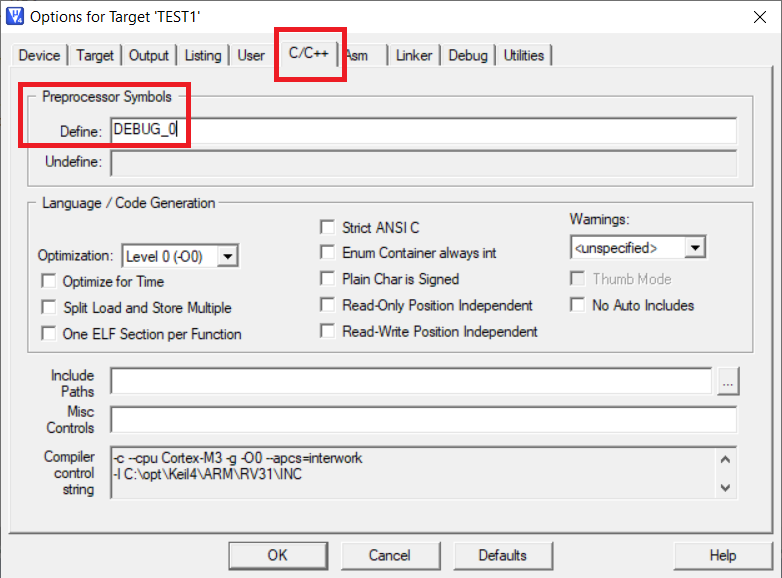
\includegraphics[width=4in]{figure/Keil_IDE_Preprocessor}}
\caption{Keil IDE: preprocessor definition} 
\label{fig_keil_ide_preprocessor}
\end{figure}


\item[{\bf Q2:}] {\bf Is it possible to trigger UART interrupts via the keyboard while debugging with the simulator? }
\item[A2:]
Yes, just type in the \verb+UART#1+ window in simulator (assuming you are programming UART0).  
If you are looking at the sample UART IRQ code on GitHub, you need to work on the SIM target in order to see IRQs under simulator. Not the RAM target.

\end{itemize}
%\section{Miscellaneous Questions}

